\setAuthor{Jaan Kalda}
\setRound{lahtine}
\setYear{2018}
\setNumber{G 8}
\setDifficulty{7}
\setTopic{Optika}

\prob{Kolmnurk}
Joonisel on kujutatud täisnurkse kolmnurga kujutis õhukeses läätses, mis on koos oma peateljega samuti ära näidatud. Kolmnurga täisnurk on märgitud punktiga. Konstrueerige kolmnurga täisnurkse tipu tegelik asukoht.
\begin{center}
	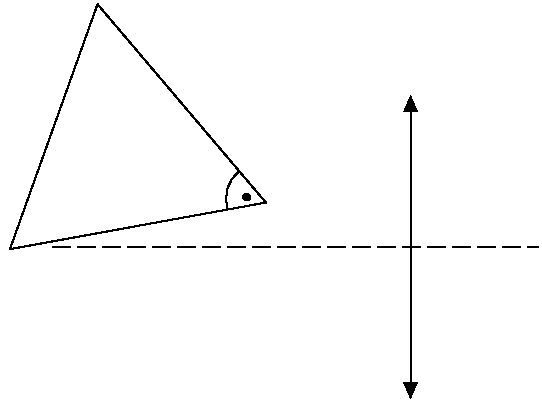
\includegraphics[width = 0.6\linewidth]{2018-lahg-08-yl.pdf}
\end{center}\hint
Paneme tähele, et sirge kujutis läbi läätse on sirge ning nende lõikepunkt on läätse tasandis. Siinkohal tuleb kasuks ka Thalese teoreem.\solu
Tähistame kolmnurga kujutise tähtedega $ABC$ (vt joonist) ja olgu täisnurkse tipu kujutisele $C$ vastav originaal punktis $F$. Paneme tähele, et sirge kujutis on sirge ning need kaks sirget lõikuvad läätse tasandis. Lõikugu küljega $AC$ määratud sirge läätse tasandiga punktis $D$ ning olgu selle sirge kujutis sirge $DF$. Analoogselt defineerime sirge 
$BC$ abil punkti $E$ ja sirge $FE$. Et $\angle DFE$ on ülesande tingimuse kohaselt täisnurk, siis peab see asuma ringjoonel, mis on ehitatud lõigule $DE$ kui diameetrile. Teisest küljest punktist $C$ läbi läätse keskpunkti tõmmatud kiir läätses ei murdu ja seetõttu peab punkt $F$ asuma sellel kiirel. Niisiis leiamegi otsitava punkti $F$ kui antud kiire ja ringjoone lõikepunkti.
\begin{center}
	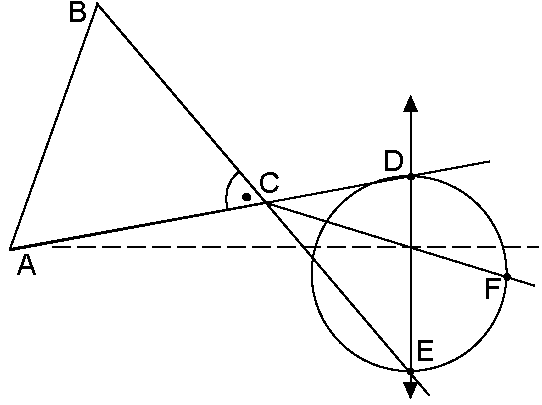
\includegraphics[width=0.5\linewidth]{2018-lahg-08-sol.pdf}
\end{center}\probend